\begin{task}{Traversing Trees}{}{}

  Trees are one of the fundamental concepts in Computer Science, Theoretically are a type of Graph,
  More specifically they are Directed Acyclic Graphs (DAGs).
  In this exercise we are getting to know traversal of a tree along the edges, a fundamental way to interact with a tree or a graph.
  More specifically we will be building recursive functions that traverse a tree in different ways.\\
  In order to do that though we first need to start understanding how to represent a tree and plot it in Matlab.\\

  We will be working with binary trees which are defined by having zero, one or two children for each node.\\ \\
  The following matlab script defines and draws a binary tree with seven
  nodes. The row vector \lstinline!nodes! defines the trees'
  nodes, by giving the index of the parent node in each element and the
  root node as 0. The values for each node of the tree are given in the
  cell array \lstinline!values!

  \begin{lstlisting}
nodes = [2 4 2 0 6 4 6];
values = {1,3,4,5,6,7,9};
treeplot(nodes);
[x,y] = treelayout(nodes);
text(x + 0.02,y,values);
\end{lstlisting}

  \begin{center}

    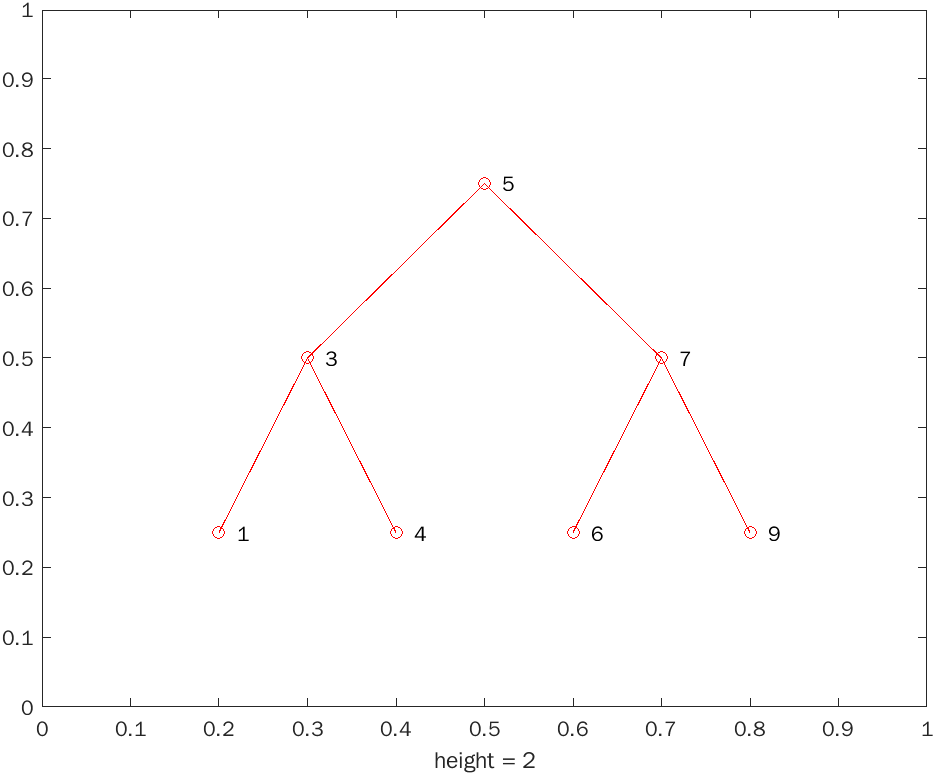
\includegraphics[width=10cm]{gfx/2021_14_tree_traversal.png}
  \end{center}

  \begin{enumerate}

    \item{\textbf{Vector
            Representation:}
          If we are careful we can represent a vector in a single vector by
          storing the root first, then the left child, then the right child, then
          the children from left to right of the next layer and so on. Empty nodes
          can represented by \lstinline!NaN! the matlab version of
          ´Nothing´: (https://www.mathworks.com/help/matlab/ref/nan.html)

          Write the vector given in the above snippet in this form.

          Implement three functions, that take a tree vector and index as input:
          \begin{enumerate}
            \item{
                  \lstinline!left_child(tree, index)!: returns a vector
                  with the value and index of the left child node or
                  \lstinline![NaN, NaN]!
                  }
            \item{
                  \lstinline!right_child(tree, index)!: returns a vector
                  with the value and index of the right child node or
                  \lstinline![NaN, NaN]!
                  }
            \item{
                  \lstinline!parent(tree, index)!: returns a vector with the
                  value and index of the parent node or \lstinline![NaN, NaN]!
                  }
          \end{enumerate}
          }

    \item{\textbf{Breadth First:}
          Using the representation and functions from \textbf{a}, write a
          recursive function \lstinline!breadth_first(tree, index)!
          that traverses the tree from the given index starting with the root and
          writes the nodes values from left to right into an output vector, before visiting nodes one layer deeper.

          You should get the following result:
          \lstinline!result = [5,3,7,1,4,6,9]!

          }

    \item{\textbf{Depth First:}
          Using the representation and functions from \textbf{a}, write a
          recursive function  \lstinline!depth_first(tree, index)!,
          that traverses the tree depth first, meaning it starts at the root and
          traverses to the bottom left of each branch first, before it backtracks to visit the
          right side on the ascent.

          You should get the following result:
          \lstinline!result = [5,3,1,3,7,6,9]!

          }

  \end{enumerate}

\end{task}
